\documentclass[11pt]{article}

\usepackage[utf8]{inputenc}
\usepackage[T1]{fontenc}
\usepackage[ngerman]{babel}
\usepackage[a4paper,margin=0.85in]{geometry}
\usepackage{graphicx}
\usepackage{array}
\usepackage{parskip}
\usepackage{ragged2e}

\pagestyle{empty}
\renewcommand{\baselinestretch}{1.0}

\begin{document}

% ---------- Title ----------
\begin{center}
    {\Large \textbf{Bewerbung}} \\[3cm]
    
    {\Huge \textbf{Zhongli Wang}} \\[0.4cm]
    
    {\huge Bewerbung als Data Scientist}
\end{center}

\vspace{0.6cm}

% ---------- Large Picture in the Middle ----------
\begin{center}
    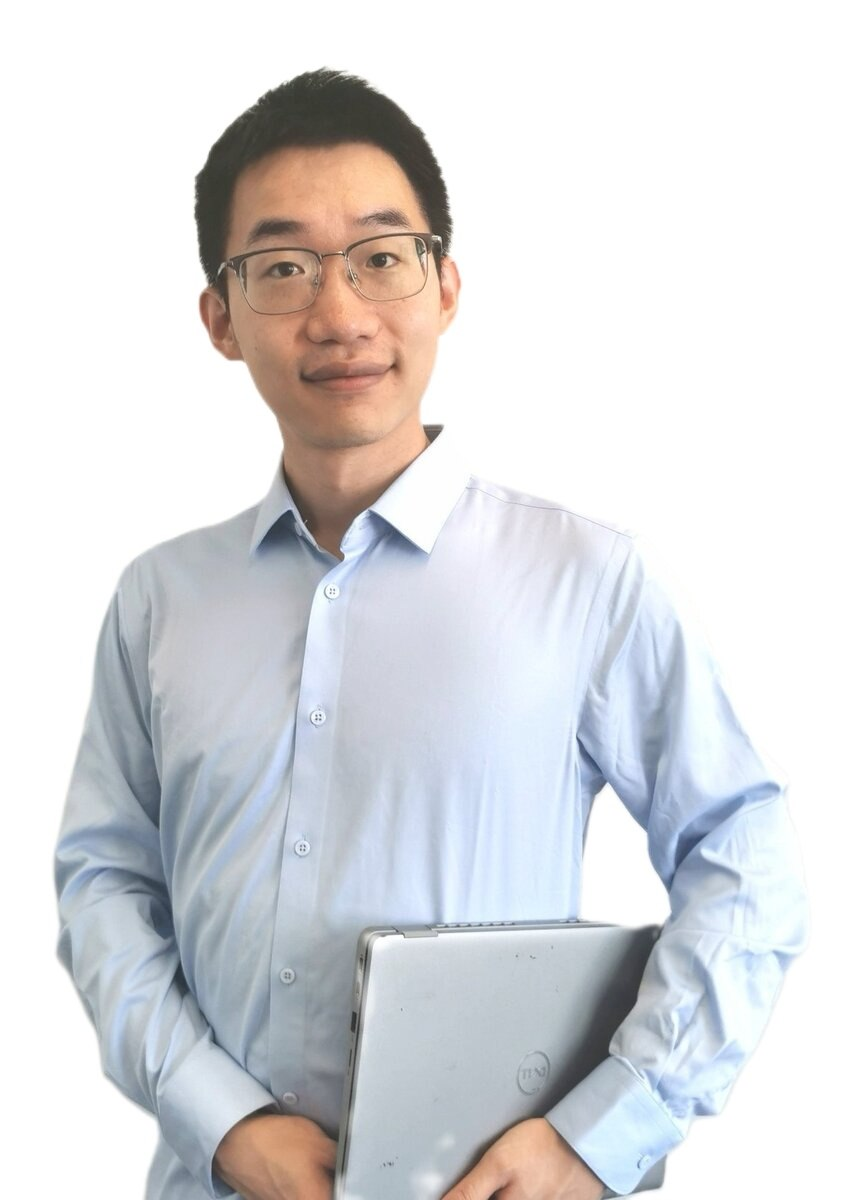
\includegraphics[
        width=0.55\textwidth,
        height=0.45\textheight,
        keepaspectratio
    ]{../zhongli-wang-profile.jpg}
\end{center}

\vspace{0.7cm}

% ---------- Personal Details ----------
\begin{center}
\renewcommand{\arraystretch}{1.35}
\begin{tabular}{>{\bfseries}p{4.2cm} p{8.5cm}}

Anschrift: & Astastrasse 22, 33617 Bielefeld, Deutschland \\

Telefon: & +49 160 9541 6015 \\

E-Mail: & nkwangzhongli@gmail.com \\

\end{tabular}
\end{center}

\vfill

\newpage

\begin{flushright}
Zhongli Wang \\
Astastrasse 22 \\
33617 Bielefeld \\
Deutschland \\
\end{flushright}

\vspace{0.1cm}

\noindent
Recruiting-Team \\
MEAG \\
München, Deutschland \\

\vspace{0.05cm}

\noindent
\textbf{Bewerbung als Data Scientist} 

\noindent Sehr geehrtes Recruiting-Team,

ich schlie\ss{}e derzeit meine Promotion in Wirtschaftswissenschaft an der Universität Bielefeld ab (Abschluss September 2026). 
Meine Forschung verbindet quantitative ökonomische Modellierung, Datenanalyse, Simulationen und empirische Methoden. Die Position als Data Scientist bei MEAG interessiert mich sehr, da sie mir die Möglichkeit bietet, meine Fähigkeiten in Datenanalyse, maschinellem Lernen und technischer Umsetzung einzubringen, um AI-Transformation in einem führenden Asset-Management-Unternehmen voranzutreiben.

Mein Hintergrund qualifiziert mich besonders für diese Rolle: Ich habe komplexe wirtschaftliche und geschäftliche Probleme strukturiert, Lösungskonzepte entwickelt und diese implementiert. Im Rahmen meiner Promotion habe ich agentenbasierte Modelle zur Analyse von Wettbewerbsdynamiken und Investitionsentscheidungen entwickelt und validiert. Ich habe Python-basierte Prototypen und Produktionssysteme gebaut, die Datenverarbeitung, maschinelles Lernen (XGBoost, Random Forest, Neural Networks) und statistische Analyse kombinieren. Gleichzeitig habe ich komplexe ökonomische Konzepte in klare, entscheidungsrelevante Erkenntnisse für unterschiedliche Zielgruppen übersetzt.

Meine technischen Fähigkeiten umfassen Python (pandas, NumPy, scikit-learn), SQL, statistische Modellierung und maschinelles Lernen. Ich habe Erfahrung mit LLMs, Prompt Engineering und agentenbasierten Workflows. Meine Stärke liegt darin, zwischen strategischen Überlegungen und praktischer Umsetzung zu wechseln: Ich kann Business-Anforderungen analysieren, AI-Use-Cases strukturieren, Prototypen entwickeln und Lösungen in bestehende Prozesse integrieren.

MEAG ist für mich besonders attraktiv, weil ich in einem Umfeld arbeiten möchte, in dem AI-Transformation strategisch und verantwortungsvoll vorangetrieben wird. Ich bin motiviert, Business-Units bei der Identifikation von AI-Chancen zu beraten, Use-Cases zu strukturieren, Projekte zu leiten und Teams bei der praktischen Anwendung von AI zu unterstützen. Meine Erfahrung in Finanzanalyse, Risikomanagement und datengestützter Entscheidungsfindung wird mir helfen, die spezifischen Anforderungen des Asset-Management-Kontextes zu verstehen.

Ich freue mich sehr, in einem persönlichen Gespräch zu erläutern, wie meine Fähigkeiten zur AI-Transformation bei MEAG beitragen können.

\vspace{0.15cm}

\noindent Mit freundlichen Grü\ss{}en, \\
\vspace{2mm}\\
\noindent Zhongli Wang

\vspace{0.05cm}
\noindent
\includegraphics[width=2.7cm,keepaspectratio]{../Wang-sig.jpg}

\end{document}
